\chapter{Implementation}
% This chapter should describe what was actually produced: the programs which were written, the hardware which was built or the theory which was developed. Any design strategies that looked ahead to the testing stage might profitably be referred to (the professional approach again).
% Descriptions of programs may include fragments of high-level code but large chunks of code are usually best left to appendices or omitted altogether. Analogous advice applies to circuit diagrams.
% Draw attention to the parts of the work which are not your own. The Implementation Chapter should include a section labelled ”Repository Overview”. The repository overview should be around one page in length and should describe the high-level structure of the source code found in your source code Repository. It should describe whether the code was written from scratch or if it built on an existing project or tutorial. Making effective use of powerful tools and pre-existing code is often laudable, and will count to your credit if properly reported.
% It should not be necessary to give a day-by-day account of the progress of the work but major milestones may sometimes be highlighted with advantage.

Could be split into \textit{preprocessing, parameter tuning, evaluation framework, software engineering techniques, repository overview}

\subsection{Precomputation and preprocessing of connectivity matrices}
Tangent works better than correlation or partial correlation.

\subsection{Structural and functional data extraction}


\subsection{Graph construction pipeline}

\begin{figure}[!ht]
    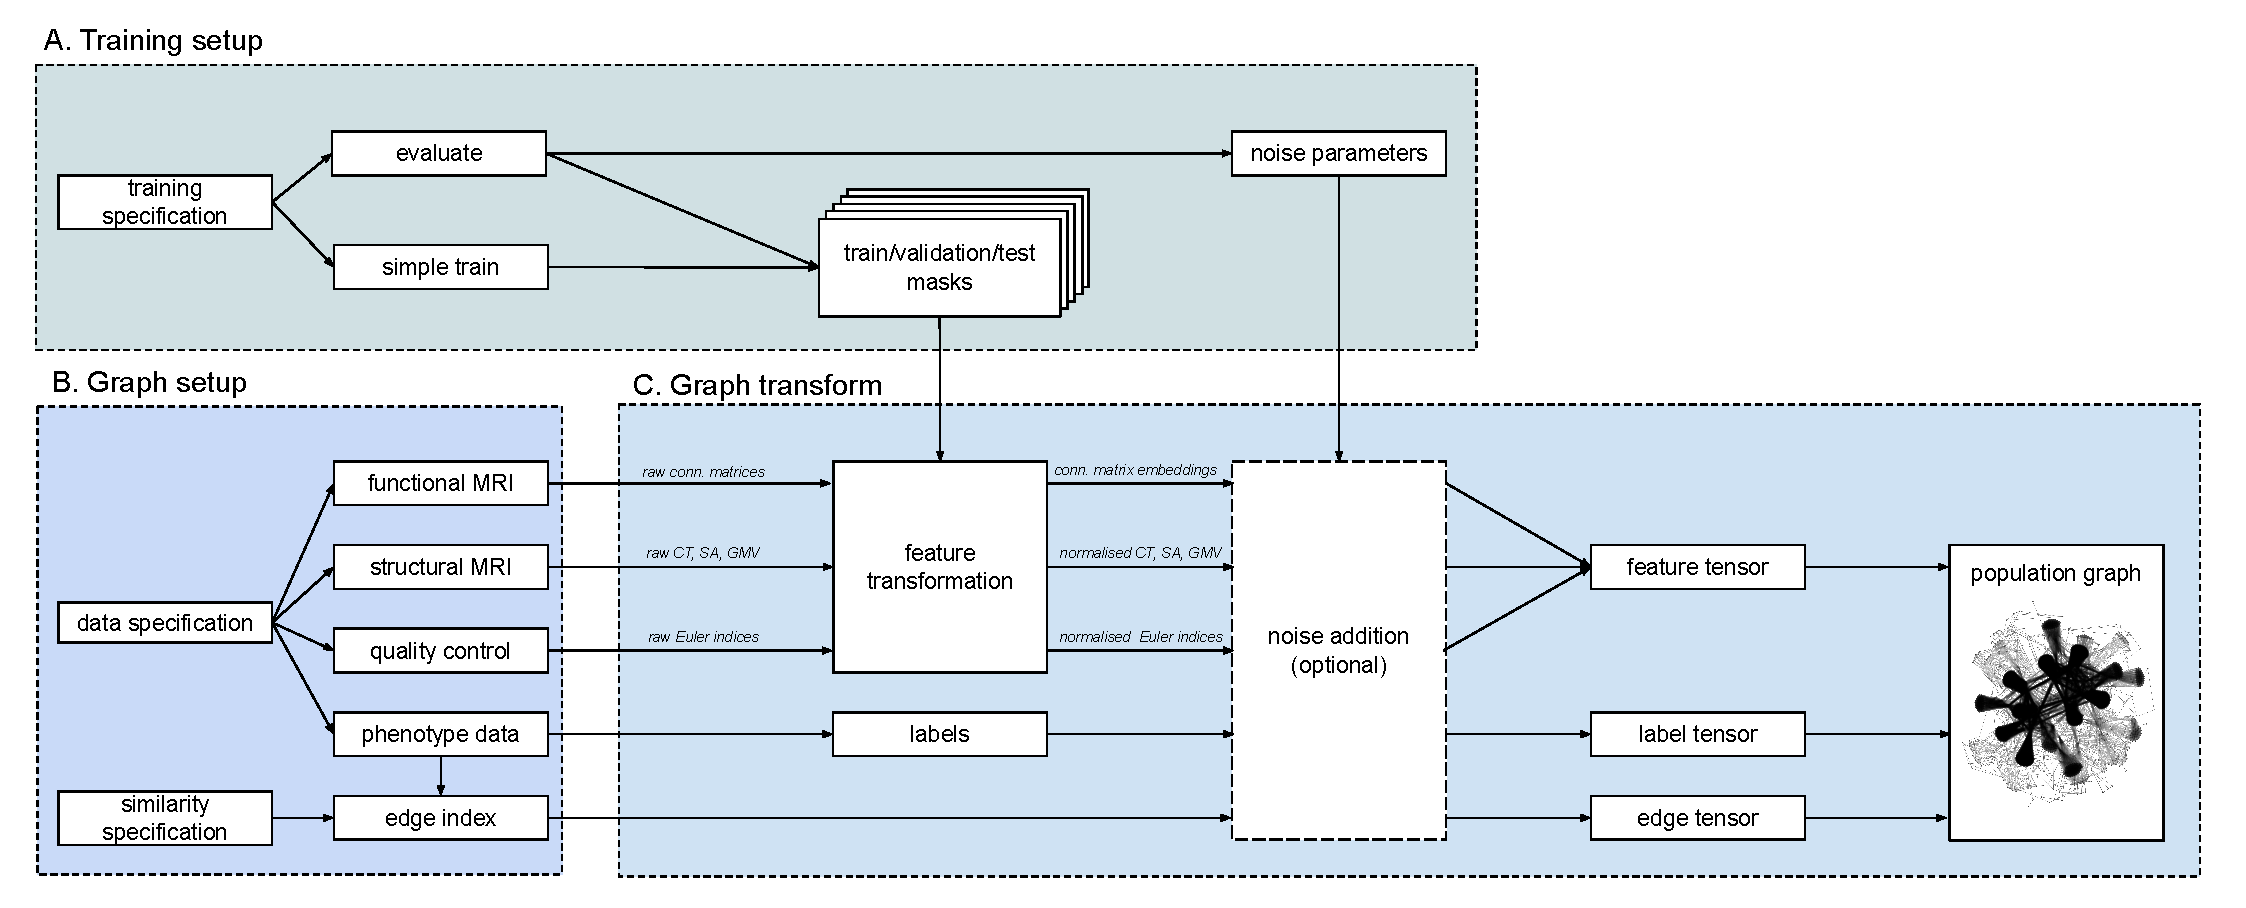
\includegraphics[width=\textwidth]{graphpipeline.pdf}
    \label{graphpipeline}
    \caption{Graph pipeline.}
\end{figure}

\subsection{Train, test, validation split}

\section{Non-graph baselines}
I have played around with \textit{xgboost}, ElasticNet and simple multilayer perceptrons to get a good idea of the minimum baselines my new architectures need to reach to be considered more effective.

\section{Graph convolutional network}
Describe the architecture in \texttt{BrainGCN}

\section{Graph attention network}

\section{Robustness evaluation framework}

\section{Repository overview}
Figure out how to split framework modules.

Could have a base BrainGNN class which can then be \textit{extended} with BrainGAT, BrainGCN.
